%% Submissions for peer-review must enable line-numbering 
%% using the lineno option in the \documentclass command.
%%
%% Camera-ready submissions do not need line numbers, and
%% should have this option removed.
%%
%% Please note that the line numbering option requires
%% version 1.1 or newer of the wlpeerj.cls file, and
%% the corresponding author info requires v1.2


\documentclass[fleqn,10pt,lineno]{wlpeerj}
\usepackage{wasysym} %% for male & female symbols
\usepackage{hyperref}
\usepackage{natbib}


%-----------------------------------------
%----- Extra packages to use Markdown 
\usepackage[footnotes,definitionLists,hashEnumerators,smartEllipses, hybrid]{markdown}

% define your color
\definecolor{my_url}{RGB}{51, 122, 183}

%  remove enumeration from headings
\setcounter{secnumdepth}{0} 

%  set up color options for links
\hypersetup{
    colorlinks=true,
    linkcolor=purple,
    filecolor= purple,
    citecolor=purple,
    urlcolor=my_url,
    % pdftitle={Overleaf Example},
    pdfpagemode=FullScreen,
    }

%  make markdown url links colored
\markdownSetup{
renderers={
  link = {\href{#3}{#1}}
}}
%-----------------------------------------



\title{Review of \textit{Amietina} (Coleoptera: Scarabaeinae: Onthophagini) with semantic descriptions of two new species from the Eastern Arc Mountains}

\author[1,2]{Giulio Montanaro}
\author[1]{Sergei Tarasov}
\affil[1]{Finnish Museum of Natural History, Pohjoinen Rautatiekatu 13, FI-00014 Helsinki, Finland}
\affil[2]{Association Catharsius, Paris, France}
\corrauthor[1]{Giulio Montanaro}{giuliomontanaro98@gmail.com}

% \keywords{Keyword1, Keyword2, Keyword3}

\begin{abstract}
The taxonomy and systematics of the genus \textit{Amietina} Cambefort, 1981 are reviewed. Two new species from the Eastern Arc Mountains (Tanzania), \textit{Amietina grebennikovi} n. sp. and \textit{Amietina mazumbaiensis} n. sp., are described and illustrated. The morphological definition of the genus is revised and expanded with the inclusion of novel characters from male genitalia. Species descriptions are made computable using the semantic language Phenoscript, and nanopublications are used to share new taxon statements. Lastly, the use of some homologous characters in Onthophagini systematics, as well as some biogeographic aspects about the new species, are discussed. ???
\end{abstract}

\begin{document}

\flushbottom
\maketitle
\thispagestyle{empty}

\section*{Introduction}

The hyperdiverse dung beetle tribe Onthophagini (Coleoptera: Scarabaeidae: Scarabaeinae) comprises almost 3000 described species \citep{schoolmeesters2021scarabs}. The majority of them has antennae with 9 segments \citep{cambefort1981amietina}. Yet, several genus-group taxa featuring only 8 antennomeres have been described: \textit{Amietina} Cambefort, 1981 (4 spp.), \textit{Cleptocaccobius} Cambefort, 1984 (24 spp.), \textit{Hathoronthophagus} Stals, Daniel \& Deschodt, 2024 (1 sp.), \textit{Megaponerophilus} Janssens, 1949 (1 sp.), \textit{Unidentis} Josso \& Prévost, 2008 (1 sp.), and other 13 genera belonging to the \textit{Stiptopodius}-group \citep{branco1989etude, branco1992essai, schoolmeesters2021scarabs} (62 spp.). The same character is also found in several species of \textit{Caccobius} (\textit{Caccophilus}) Jekel, 1872 \citep{cambefort1979donnees}, \textit{Onthophagus} (\textit{Furconthophagus}) Zunino, 1979 (\citealp{cambefort1986une}; GM, personal observation) and \textit{Onthophagus} (\textit{sensu lato}) Latreille, 1802 (\citealp{cambefort1981amietina}; GM, personal observation). 

The genus \textit{Amietina} is characterised, in addition to the 8-segmented antennae, by the following characters: 1) the absence of a 4\textsuperscript{th} tooth on the protibial margin; 2) the distal protibial margin most often perpendicularly truncated; 3) the presence of a small tooth in the distoventral margin of male protibiae; 4) the bidentate clypeus; 5) the absence of any head protrusion except for a blunt, transverse gibbosity; and 6) the body small and lenticular \citep{branco1988deux, cambefort1981amietina}. Although most if not all of these traits are homoplasious in the Onthophagini (\citealp{philips2016phylogeny}; \citealp{tarasov2011phylogenetic}), their combination is unique within the tribe and makes the genus easily identifiable. \textit{Amietina} currently comprises four described species, two of them found in West and Central-West African forests (\textit{A. larrochei} Cambefort, 1981 and \textit{A. eburnea} Cambefort, 1981), one in Uganda (\textit{A. cambeforti} Branco, 1988) and one in Malawi (\textit{A. nyassalandica} Branco, 1988) \citep{branco1988deux, cambefort1981amietina}.

During our ongoing survey of the dung beetle fauna of the Eastern Arc Mountains (Tanzania), we found two undescribed, very closely allied species of Onthophagini occurring in the rainforests of the West Usambara and the Udzungwa Mountains. The only female specimen available almost perfectly matches the diagnostic features of \textit{Amietina}. However, males do not completely fit the definition of the genus, as they have the apex of protibiae obliquely truncated (perpendicularly truncated in \textit{Amietina}) and the head bearing a tubercle.

In which (sub)genus should these species be included? To understand it, we studied the morphology of all described \textit{Amietina}, including phylogenetically informative characters of male genitalia that were never employed before. Our examination led us to define a new set of diagnostic characters of \textit{Amietina sensu novo}, in which we accommodate the two new taxa from Tanzania -- \textit{Amietina grebennikovi} n. sp. and \textit{Amietina mazumbaiensis} n. sp. The description of the unknown female of \textit{Amietina nyassalandica} and an identification key to all the species are also provided. Additionally, we discuss the usefulness and the limits of some morphological characters previously used to define \textit{Amietina} in the broader context of Onthophagini systematics.  Lastly, we emphasize that the new taxa represent another probable case of single-block endemism in the Eastern Arc Mountains.

Taxonomic descriptions are written with Phenoscript, an emerging semantic language for making phenotypic data easily computer-parsable that has already been successfully implemented in insect taxonomy (\citealp{miko2021semantically, montanaro2024beyond, montanaro2024computable}). Additionally, the new species names are published online in the form of nanopublications, \textit{quanti} of information easily searchable and retrievable from the web \citep{kuhn2013broadening, montanaro2024beyond}. These two tools make the taxonomic information disclosed by this work compliant with \href{https://www.go-fair.org/fair-principles/}{FAIR} principles of Findability, Accessibility, Interoperability and Reusability, thus enhancing the potential reuse of our data for future applications.

\section*{Materials and Methods}

\subsection*{Specimens examination}
According to the identification key by \cite{orbigny1913synopsis} on African Onthophagini, the two new species could belong to the \textit{Onthophagus} groups 2 or 3. To understand whether they had already been described or not, we compared them with the descriptions of all known species in groups 2 (REFS) and 3 \citep{daniel2023dung}.

Specimens of all known \textit{Amietina} species were examined. We studied only a female of \textit{A. nyassalandica}; male characters were retrieved from the detailed original description by \cite{branco1988deux}. Part of the specimens of \textit{A. cambeforti}, \textit{A. eburnea} and \textit{A. larrochei} come from the same collecting events of those examined by \cite{branco1988deux}. 
All specimens are preserved at the Finnish Museum of Natural History Luomus (Helsinki, Finland; initialism: MZH), in the collection of the first author (Creazzo, Italy; initialism: GMOC) and in Jean-Fran\c{c}ois Josso's private collection (Muzillac, France; initialism: JFJC). Holotypes and paratypes of the new species are all preserved in MZH.

An additional specimen from the Rubeho Mountains putatively attributable to \textit{Amietina sensu novo} was identified among the samples registered in the \href{https://boldsystems.org/}{Barcode of Life Database} (BOLD) (unique ID: \href{https://boldsystems.org/index.php/Public_RecordView?processid=VGH254-12}{CNCCOLVG00004064}) by the colleague Vasily Grebennikov (Canadian Food Inspection Agency, Ottawa, Canada). However, despite the kind efforts of V. Grebennikov and Bruce Gill (Canadian National Collection of Insects, Ottawa, Canada), it was not possible to locate the physical voucher, which shall be considered lost. Unfortunately, the only available picture is not sufficient to diagnose the species, that therefore will not be treated here.

Morphological terminology and protocols follow \cite{montanaro2024computable} and \cite{tarasov2011phylogenetic}. The map was realised in QGIS \citep{QGIS_software} and Eastern Arc forests outlined using the Terrestrial Ecoregions of the World layer \citep{olson2001terrestrial}. Figures were edited in Adobe Photoshop and Adobe Illustrator.

For holotype labelling, we use “//” to separated different labels and “/” to separate lines on the same label. Comments to labels are enclosed in square brackets.

\subsection*{Semantic descriptions and nanopublications}

Morphology was described using the semantic language \href{https://github.com/sergeitarasov/PhenoScript}{PhenoScript}, which uses terms from anatomy ontologies to build computer-parsable taxonomic descriptions. We follow the workflow developed in previous papers \citep{montanaro2024beyond, montanaro2024computable}.

In \textit{Amietina}, the distoventral margin of the protibia of males bears a sharp cuticular spine. This structure is present, with different degrees of development, also in males of many other Scarabaeinae – {\textit{e.g.}}, the whole tribe Onitini \citep{janssens1937revision}, many Deltochilini \textit{sensu lato}, the genera \textit{Catharsius} Hope, 1837 and \textit{Metacatharsius} Montreuil, 1998 \citep{scholtz1987revision, tarasov2015innovative}, other Onthophagini lineages such as \textit{Proagoderus} Lansberge, 1883 \citep{palestrini1992sistematica}, \textit{Digitonthophagus} Balthasar, 1959 \citep{genier2017digitonthophagus}, \textit{Onthophagus} (\textit{Furconthophagus}) Zunino, 1979 (GM, personal observation), \textit{etc}. Similar structures also exist in other Scarabaeoidea, for example in the Euchirinae \citep{young1989euchirinae} and in some Cetoniinae Goliathini \citep{de2024taxonomic}. Traditionally, many words have been used to refer to this spine in Scarabaeinae: ``éperon" \citep{janssens1937revision}, ``finger-like process" \citep{krikken1977notes}, ``tooth" \citep{genier2019new}, ``internoapical tooth" \citep{genier2017digitonthophagus}, ``denticule apical interne" \citep{dierkens2023gonionthophagus}, ``spur" \citep{scholtz1987revision}, \textit{etc}. This plethora of terms is often used to also indicate different structures, like the flat protrusions on the dorsal margin of protibia, which we proposed to call \href{https://ontobee.org/ontology/AISM?iri=http://purl.obolibrary.org/obo/AISM_0000366}{protibial teeth} \citep{montanaro2024computable}, or the articulated spine in the distal edge of protibia, which shall be called \href{https://ontobee.org/ontology/AISM?iri=http://purl.obolibrary.org/obo/AISM_0000040}{spur} \citep{giron2024AISM}. Here, we propose that \href{https://ontobee.org/ontology/COLAO?iri=http://purl.obolibrary.org/obo/COLAO_0000038}{\textit{uncus}} (COLAO:0000038), Latin for ``hook", could become the standard term to be consistently used in scarabaeine taxonomy to refer specifically to the protibial distoventral spine. This term is unambiguously defined in the Coleoptera Anatomy Ontology (COLAO), currently the largest and most curated dictionary for beetle anatomical terminology available online \citep{giron2024colao}. Although, to our knowledge, \textit{uncus} was never used for dung beetles, it is already employed in other beetle taxa \citep{lawrence2013australian}. For similar structures located on meso- and metalegs, much rarer in Scarabaeinae, for now we suggest to maintain the more general term ``cuticular spine" (see also \citep{montanaro2024beyond}).

As mentioned above, the \textit{uncus} must not be mistaken with the protibial spur, which is articulated. However, in at least the case of Onitini, the \textit{uncus} may have originated by fusion of the protibial spur (now undistinguishable in males), either with the tibial margin, or with the protibial margin plus a pre-existing \textit{uncus}. This hypothesis is supported by the observation that in some Onitini (\textit{e.g.}, \textit{Onitis punctatostriatus} Janssens, 1937), an unarticulated spur-like protrusion is fused to the main body of the \textit{uncus}, suggesting a fusion of the spur rather than its loss (GM, personal observation). This raises questions about how to take into account this putatively partial homology relationship between spur and spine in Onitini when writing descriptions with Phenoscript. However, we postpone this question to possible future works dealing with Onitini, not being the aim of this paper.

Statements on the establishment of the new species names were published, in addition to the regular Zoobank registration, in the form of nanopublications. Nanopubs were realised in \href{https://nanodash.petapico.org/publish?}{nanodash} using the \href{https://nanodash.petapico.org/publish?11&template=https://w3id.org/np/RAa7sIgQ77jJL4HYYGVH8sNu1YEKCH3F-CHqHrgbWWGS4}{format for defining new taxa} already tested by \cite{montanaro2024beyond}.


\section*{Taxonomy}

\subsection*{\textit{Amietina} Cambefort, 1981}

\cite{cambefort1981amietina}: 143 (original description);\\
\cite{cambefort1984etude}: 106 (ecology);\\
\cite{cambefort1985coleopteres}: 339 (faunistics);\\
\cite{branco1988deux}: 201 (description of 2 new species);\\
\cite{nummelin1989dung}: 351 (ecology);\\
\cite{cambefort1991dung}: 200 (ecology);\\
\cite{cambefort2003nimba}: 559 (faunistics);\\
\cite{davis2008african}: 216 (systematics, natural history);\\
\cite{josso2008unidentis}: 2 (systematics);\\
\cite{moretto2010bayanga}: 469 (faunistics);\\
\cite{moretto2010onthophagus}: 14 (ecology, natural history);\\
\cite{branco2014scarabaeidae}: 11 (nomenclature);\\
\cite{philips2023dung}: 2 (ecology).


\textbf{Type species}: \textit{Amietina larrochei} Cambefort, 1981 (by original designation).

\textbf{Diagnosis}. The genus is a member of the tribe Onthophagini. It can be differentiated from all other genera and subgenera of \textit{Onthophagus} by the following combination of characters: 1) body small (3.2--5.0mm), lenticular; 2) antennae with 8 segments; 3) clypeus with two teeth; 4) protibiae with 3 teeth on dorsal margin (\textbf{Fig}. \ref{fig:fig1}e--h); 5) male protibiae with a small, sharp \textit{uncus} (\textbf{Fig}. \ref{fig:fig1}e,g--h); 6) dorsal body surface covered with simple punctures bearing conspicuous setae; 7) parameres acuminate and bent posteroventrally (\textbf{Fig}. \ref{fig:fig2}a,d,g,i,k); 8) lamella copulatrix composed by two separate endophallites somehow arranged in a circle, plus an additional, elongated small distal endophallite (\textbf{Fig}. \ref{fig:fig2}l--n). 
The following two characters, previously used to define the genus, are here reconsidered: 1) head surface either devoid of protrusions (but often with a transverse bulging on the frons), or, in males of \textit{A. mazumbaiensis} \textbf{n. sp.} and \textit{A. grebennikovi} \textbf{n. sp.}, with a small frontal tubercle; 2) distal protibial margin either perpendicularly truncated, or, in the new species and in the female of \textit{A. larrochei}, obliquely truncated (\textbf{Fig}. \ref{fig:fig1}e--h).

\textbf{Distribution}. The genus is endemic to the Afrotropical region.

\textbf{Ecology}. Based on literature \citep{branco1988deux} and the present data, \textit{Amietina} species are forest-specialised. Most species are found in evergreen rainforests, the only exception being \textit{A. nyassalandica}, which was found in miombo woodlands. Specimens were collected in ant nest debris, excrements, rotten fish, fruits and dead diplopods, suggesting a rather generalist feeding behaviour \citep{branco1988deux, moretto2010onthophagus}.

\textbf{Remarks}. Based on morphology, the genus can be subdivided into two operational species-groups:
\begin{enumerate}
    \item \textit{Amietina larrochei} species-group, characterized by: 1) absence of protrusions on the head of both sexes, surface at most swollen medially; 2) male protibiae perpendicularly truncated distally; 3) proximal region of endophallus without raspulae.
    \item \textit{Amietina mazumbaiensis} species-group, characterized by: 1) presence of a tubercle on male head; 2) distal edge of protibiae obliquely truncated; 3) proximal region of endophallus with raspulae.
\end{enumerate}

\textbf{Species included}:

\smallskip \noindent \textbf{\textit{A. larrochei} species-group}:

\indent \textit{A. cambeforti} Branco, 1989 (Uganda);

\indent \textit{A. larrochei} Cambefort, 1981 (Cameroon, Gabon, Liberia);

\indent \textit{A. eburnea} Cambefort, 1981 (Ivory Coast, Guinea, Liberia);

\indent \textit{A. nyassalandica} Branco, 1989 (Malawi);

\smallskip \noindent \textbf{\textit{A. grebennikovi} species-group}:

\indent \textit{A. grebennikovi} \textbf{n. sp.} (Tanzania);

\indent \textit{A. mazumbaiensis} \textbf{n. sp.} (Tanzania);

\smallskip

Other described and undescribed species may also belong to the genus as defined here (\citealp{moretto2010onthophagus}; P. Moretto, personal communication) (see also the Discussion).


\subsection*{\textbf{\textit{Amietina grebennikov test !!!!!} Branco, 1989}}
(Figs. \ref{fig:fig2}k)\\
\cite{branco1988deux}: 201 (original description);\\
\cite{nummelin1989dung}: 351 (ecology, as ``{Amietina} n. sp.");\\
\cite{davis2008african}: 216 (systematics, natural history);\\


\markdownInput{Amietina_grebennikovi_test.md}






\subsection*{\textbf{\textit{Amietina cambeforti} Branco, 1989}}
(Figs. \ref{fig:fig2}k)\\
\cite{branco1988deux}: 201 (original description);\\
\cite{nummelin1989dung}: 351 (ecology, as ``{Amietina} n. sp.");\\
\cite{davis2008african}: 216 (systematics, natural history);\\

\textbf{Type locality:} Kibale Forest (Uganda).

\textbf{Material examined (xx\male\male, xx\female\female).} \textbf{UGANDA}: W Province, Kibale forest, Ngogo, 6.iv.1984, M. Nummelin \textit{legit} [2 exx, MZH].

\textbf{Diagnosis.} This species belongs to the \textit{A. larrochei}-group. See \citep{branco1988deux} and the identification key below for further details.

\textbf{Distribution:} Uganda \citep{branco1988deux}.

\subsection*{\textbf{\textit{Amietina eburnea} Cambefort, 1981}}
(Figs. \ref{fig:fig1}g, \ref{fig:fig1}i--j) \\
\cite{cambefort1981amietina}: 143 (original description);\\
\cite{cambefort1984etude}: 106 (ecology);\\
\cite{cambefort1985coleopteres}: 339 (faunistics);\\
\cite{branco1988deux}: 201 (taxonomy);\\
\cite{cambefort1991dung}: 405 (ecology);\\
\cite{cambefort2003nimba}: 559 (ecology);\\
\cite{davis2008african}: 216 (systematics, natural history);\\
\cite{moretto2010bayanga}: 469 (faunistics);\\

\textbf{Type locality:} Bandama gallery forest, Lamto (Ivory Coast).

\textbf{Material examined (xx\male\male, xx\female\female).} \textbf{LIBERIA}: Mt. Nimba, grassfield, 16-25.ix.1979, lowland forest, 500m, fish trap, I. Hanski \textit{legit} [5 exx, MZH].

\textbf{Diagnosis.} This species belongs to the \textit{A. larrochei}-group. See \citep{branco1988deux} and the identification key below for further details.

\textbf{Distribution:} Ivory Coast \citep{cambefort1981amietina}, Guinea \citep{cambefort2003nimba}, Liberia \citep{branco1988deux}.


\subsection*{\textbf{\textit{Amietina grebennikovi} n. sp.}}
(Figs. \ref{fig:fig1}c, \ref{fig:fig2}d--f, \ref{fig:fig2}m, \ref{fig:fig3})\\

\textbf{Type locality:} Udzungwa Mountains (Tanzania).

\textbf{Material examined. Holotype (\male):} Tanzania, Udzungwa Mts., -7.845 36.8761, 454m, 6.x.2014, sift2, V. Grebennikov \textit{legit}. \textbf{Paratype (\male):} \textit{idem} holotype [MZH].

\textbf{Diagnosis}. \textit{Amietina grebennikovi} n. sp. belongs to the \textit{A. mazumbaiensis}-group as defined above. Externally, it is almost undistinguishable from \textit{A. mazumbaiensis} n. sp. The only conspicuous differences observed are the... 
However, these differences must be taken cautiously, given that variation in the two species is virtually unknown due to the very limited number of examined specimens. Male genitalia offer useful diagnostic characters: 1) parameral margin more strongly concave and apex more strongly curved ventrally in \textit{A. mazumbaiensis} (Fig. \ref{fig:fig2}a) than in \textit{A. grebennikovi} (Fig. \ref{fig:fig2}d); 2) in \textit{A. mazumbaiensis}, posterolateral margin of paramere notched, apex directed laterally (Fig. \ref{fig:fig2}b), while in \textit{A. grebennikovi} the distolateral margin is at most a little sinuous and the apex not directed laterally (Fig. \ref{fig:fig2}e); 3) presence of 3 distinct endophallic raspulae in \textit{A. grebennikovi} (Fig. \ref{fig:fig2}f), only 2 in \textit{A. mazumbaiensis} (Fig. \ref{fig:fig2}c); 4) endophallite 1 of lamella copulatrix with a pointed anterior projection in \textit{A. mazumbaiensis} (Fig. \ref{fig:fig2}l), simple in \textit{A. grebennikovi} (Fig. \ref{fig:fig2}m).

???? how to indicate the position of endophallites? everted or not?

\textbf{Description. Male.} Body lenticular, black, shiny, covered with pale yellowish setae. \textbf{Length:} 4.3 mm. \textbf{Head.} Subpentagonal, tapering anteriorly; anterior margin of clypeus with two teeth separated by an obtuse angle; entirely covered with simple punctures; punctures separated by approximately 1 diameter posteriorly, denser, deeper and almost rugose anteriorly. Frons bearing a transverse tubercle placed between the anterior margins of eyes. Antennae with 8 segments. \textbf{Pronotum.} Maximum width in correspondence of posterolateral angles; base finely bordered laterally and medially; posterolateral angles sinuated in lateral view; covered with simple setigerous punctures intermixed with smaller ones, the largest ones separated by approximately 2 diameters on disc. \textbf{Elytra.} Wider than pronotum; striae clearly impressed, in number of 8; strial punctures distinctly larger than strial width; interstriae punctured, punctures roughly disposed in 2 rows on disc; scutellum absent. \textbf{Tergite VIII.} Cuticular punctures simple, deep, separated by approximately 1 diameter.  \textbf{Inferior body surface.} Anterior region of hypomera concave; hypomeral carina directed toward lateral pronotal edge before curving toward anterior angle. \textbf{Legs}. Protibiae with three external teeth; distal edge oblique, with a small sharp tooth close to protarsal insertion. Anteroventral carina of profemora entire. \textbf{Genitalia.} Parameres elongated, apices sharp and bent ventrally in lateral view (Figs. \ref{fig:fig2}d); parameral margin not notched posterolaterally (Fig. \ref{fig:fig2}e). Endophallus with 3 clearly sclerified raspulae (Fig. \ref{fig:fig2}f); endophallite 1 of lamella copulatrix simple anteriorly (Fig. \ref{fig:fig2}m).

\textbf{Female.} Unknown.

\textbf{Variation.} No significant variation was observed.

\textbf{Etymology.} We are glad to dedicate this new species to his collector, the colleague Vasily V. Grebennikov, who has been sampling arthropods extensively in the Eastern Arc Mountains using soil sifting. His efforts with this challenging technique have already disclosed extremely interesting dung beetle species.

\textbf{Distribution and ecology.} The new species was collected in the forest of the Udzungwa Mountains (Map \ref{fig:fig3}), by sifting litter. Similarly to other \textit{Amietina} (see above), it may have non-strictly coprophagous habits such as saprophagy and/or necrophagy.

\subsection*{\textbf{\textit{Amietina larrochei} Cambefort, 1981}}
(Figs. \ref{fig:fig1}d, \ref{fig:fig1}h, \ref{fig:fig1}g--h, \ref{fig:fig1}n) \\
\cite{cambefort1981amietina}: 143 (original description);\\
\cite{branco1988deux}: 201 (taxonomy);\\
\cite{cambefort1991dung}: 408 (ecology);\\
\cite{cambefort2003nimba}: 559 (faunistics);\\
\cite{davis2008african}: 216 (systematics, natural history);\\
\cite{moretto2010bayanga}: 469 (faunistics);\\
\cite{branco2014scarabaeidae}: 11 (nomenclature);\\

\textbf{Type locality:} Mount Kala (Cameroon).

\textbf{Material examined (xx\male\male, xx\female\female).} \textbf{CAMEROON}: Mt. Kupe, 4.8213 9.7064, 1501m, 29.xii.2015, siftCM12, V. Grebennikov \textit{legit} [2 exx, MZH]; Mt. Cameroon, 4.1175 9.0718, 1079m, 28.xii.2015, siftCM07, V. Grebennikov legit [5 exx, MZH; x exx, GMOC]. \textbf{LIBERIA}: Mt. Nimba, grassfield, 16-25.ix.1979, lowland forest, 500m, fish trap, I. Hanski \textit{legit} [5 exx, MZH].

\textbf{Diagnosis.} This species belongs to the \textit{A. larrochei}-group. See \citep{branco1988deux} and the identification key below for further details.

\textbf{Distribution:} Cameroon \citep{cambefort1981amietina}, Gabon \citep{cambefort1991dung}, Liberia \citep{branco1988deux}.

\subsection*{\textbf{\textit{Amietina mazumbaiensis} n. sp.}}
(Figs. \ref{fig:fig1}a--b, \ref{fig:fig1}e--f, \ref{fig:fig2}a--c, \ref{fig:fig2}l, \ref{fig:fig1}l) \\

\textbf{Type locality:} Mazumbai forest, West Usambara Mountains (Tanzania).

\textbf{Material examined. Holotype (\male):} Tanzania, West Usambara Mts., Mazumbai forest reserve, pitfall, 1500m, 26.xi–2.xii.1996, O. Biström, M. Nieminen, J. Terhivuo \& P. Vilkamaa \textit{legit}. \textbf{Allotype:} \textit{idem} holotype [MZH].

\textbf{Holotype labelling}: ???

\textbf{Diagnosis}. \textit{A. mazumbaiensis} n. sp. belongs to the \textit{A. mazumbaiensis}-group together with \textit{A. grebennikovi} n. sp. See diagnosis of \textit{A. grebennikovi} for further details.

\textbf{Description}. \textbf{Male}. Body lenticular, black, shiny, covered with pale yellowish setae. \textbf{Length:} 5.0 mm. \textbf{Head.} Subpentagonal, tapering anteriorly; anterior margin of epistome with two teeth separated by an obtuse angle; clypeal margin feebly and broadly sinuated at clypeogenal junction; entirely covered with simple punctures; punctures separated by approximately 1 diameter posteriorly, denser, deeper and almost rugose anteriorly. Frons bearing a transverse tubercle placed between the anterior margins of eyes. Antennae with 8 segments. \textbf{Pronotum.} Maximum width in correspondence of posterolateral angles; base finely bordered laterally and medially; posterolateral angles sinuated in lateral view; covered with sparse simple setigerous punctures intermixed with smaller ones, the largest ones separated by approximately 2 diameters on disc. \textbf{Elytra.} Wider than pronotum; striae clearly impressed, in number of 8; strial punctures distinctly larger than strial width; interstriae punctuated, punctures disposed in 2 rows on disc; scutellum absent. \textbf{Tergite VIII.} Cuticular punctures simple, deep, separated by approximately 1 diameter; surface between punctures glossy, wrinkled. \textbf{Inferior body surface.} Anterior region of hypomera concave; hypomeral carina directed toward lateral pronotal edge before curving toward anterior angle. \textbf{Legs.} Protibiae with three external teeth; distal edge oblique, with a small sharp tooth close to protarsal insertion. Anteroventral carina of profemora entire. \textbf{Genitalia.} Parameres elongated, apices sharp and bent ventrally in lateral view; apices slightly sinuated laterally in frontal view (Figs. \ref{fig:fig2}a, \ref{figure:2}b). Endophallus with 2 clearly sclerified raspulae (Fig. \ref{figure:2}e); la
XXX FINISH

\textbf{Female. Head.} Lateral margin of clypeus sinuated at clypeogenal junction; head without protrusions, only the clypeal surface slightly transversely swollen in the middle. \textbf{Pygidium.} Shorter than in the male; surface not wrinkled.

\textbf{Etymology.} The name refers to the Mazumbai Forest in the West Usambara Mounts, the only locality from which the new species is known.

\textbf{Distribution and ecology.} The new species was found in the Mazumbai forest in the West Usambara Mountains (Map \ref{fig:fig3}). Given the high rates of endemism observed in the invertebrate fauna of the Eastern Arc Mountains, it would not be surprising if it is endemic to the (West) Usambara Mountains. It was collected with pitfall traps and, similarly to other \textit{Amietina} (see above), it may have non-strictly coprophagous habits.


\subsection*{\textbf{\textit{Amietina nyassalandica} Branco, 1989}\\}

\cite{branco1988deux}: 201; (original description);\\
\cite{davis2008african}: 216 (systematics, natural history);\\
\cite{josso2008unidentis}: ??;\\

\tab\textbf{Type locality:} Chamambe Forest, Viphya Mounts (Malawi).

\textbf{Material examined (1\female).} \textbf{MALAWI}: xxx [JFJC].

\textbf{Diagnosis.} This species belongs to the \textit{A. larrochei}-group. See \citep{branco1988deux} and the identification key below for further details.

\textbf{Description of the female}. Similar to the male, except for the following features. \textbf{Length:} XXmm. \textbf{Head. Tergite VIII. }

\textbf{Distribution:} Malawi \citep{branco1988deux}.


\subsection*{Identification key to \textit{Amietina} species (translated and modified from \cite{branco1988deux})}\hspace*{1pt}
\begin{enumerate}
\item[1.] Male and female distal protibial edge oblique. Male head with a tubercle between eyes. Endophallus with raspulae\dotfill\textbf{2}
\item[--] Male and female distal protibial edge perpendicular to main tibial axis, except for the female of \textit{A. larrochei}. Male head without tubercles. Endophallus without raspulae\dotfill\textbf{3}
\item [2.] Parameral margin more strongly concave and apex more strongly curved ventrally than in the following species (Fig. \ref{fig:fig2}a). Posterolateral margin of paramere notched, apex directed laterally (Fig. \ref{fig:fig2}b). Endophallus with 2 distinct raspulae (Fig. \ref{fig:fig2}c). Endophallite 1 of lamella copulatrix with a pointed anterior projection (Fig. \ref{fig:fig2}l). Tanzania (West Usambara Mountains)\dotfill\\ .\dotfill\textbf{\textit{mazumbaiensis}} n. sp.
\item[--.] Parameral margin less strongly concave and apex less strongly curved ventrally (Fig. \ref{fig:fig2}d). Posterolateral margin of paramere at most a little sinuous, apex not directed laterally (Fig. \ref{fig:fig2}e). Endophallus with 3 distinct raspulae (Fig. \ref{fig:fig2}f). Endophallite 1 of lamella copulatrix without pointed anterior projection (Fig. \ref{fig:fig2}m). Tanzania (Udzungwa Mountains)\dotfill\textbf{\textit{grebennikovi}} n. sp.
\item[3.] Genae angled. Anterior profemoral carina restricted to the proximal 1/3. Male genitalia as in \cite{branco1988deux}. Malawi\dotfill\textbf{\textit{nyassalandica}} Branco, 1989
\item[--] Genae rounded. Anterior profemoral carina complete or interrupted by large punctures\dotfill\textbf{4}
\item[4.] Anterior profemoral carina interrupted in the middle by a row of large setigerous punctures. Male genitalia as in Figs. \ref{fig:fig2}i--j. Ivory Coast, Guinea, Liberia\dotfill\textbf{\textit{eburnea}} Cambefort, 1981
\item[--] Anterior profemoral carina complete\dotfill\textbf{5}
\item[5.] Pronotal disc with small punctures intermixed with bigger ones. Clypeus feebly sinuated (male) or moderately sinuated (female) at clypeogenal junction. Male genitalia as in Figs. \ref{fig:fig2}g--h, \ref{fig:fig2}n. Cameroon, Gabon, Liberia\dotfill\textbf{\textit{larrochei}} Cambefort, 1981
\item[--] Pronotal disc with punctures of uniform size. Clypeus not sinuated (male) or feebly sinuated (female) at clypeogenal junction. Male genitalia as in Fig. \ref{fig:fig2}k. Uganda\dotfill \\ .\dotfill\textbf{\textit{cambeforti}} Branco, 1989
\end{enumerate}


\section*{Discussion}

\subsection*{A new concept of \textit{Amietina}}
In this work we described two onthophagine species, \textit{Amietina grebennikovi} n. sp. and \textit{A. mazumbaiensis} n. sp., which fit with many but not all of the original diagnostic characters of \textit{Amietina}. Specifically, the shape of the distal margin of the protibiae and the presence of protrusions on the male heads do not match the definition of the genus given by \cite{cambefort1981amietina} and \cite{branco1988deux}. However, we believe that the importance of these external features can be downsized, as they are both very evolutionarily plastic.

The shape of the distal protibial margin is highly variable in the Onthophagini. While the ancestral condition is most likely an obliquely truncated margin, the perpendicularly truncated condition evolved many times independently \citep{ayivi2021mitochondrial, breeschoten2016phylogenetics, tarasov2011phylogenetic, philips2016phylogeny}. It is found, for example, in the polyphyletic genus \textit{Caccobius} \citep{tarasov2011phylogenetic, genier2017digitonthophagus}, in \textit{Cleptocaccobius}, \textit{Megaponerophilus}, \textit{Tomogonus} \citep{davis2008african}, \textit{Unidentis} \citep{josso2008unidentis}, \textit{Pseudosaproecius} \citep{branco1995essai}, and \textit{Onthophagus} (\textit{Furconthophagus}) (GM, personal observation). It occurs, as a male secondary sexual character, at least in \textit{Euonthophagus} and \textit{Onthophagus} (\textit{Exonthophagus}) \citep{kabakov2006scarab}, as well as in \textit{Amietina larrochei} (see above). Additionally, many taxa of the oniticelline clade of Onthophagini \citep{breeschoten2016phylogenetics} show perpendicularly truncated protibiae, including the emblematic \textit{Liatongus endroedii} Balthasar, 1956, whose sister species, \textit{Liatongus incurvicornis} (Fairmaire, 1887), has normally shaped legs \citep{balthasar1956einige}. Lastly, several taxa show intermediates between the two conditions -- \textit{e.g.}, at least some species of \textit{Onthophagus} (\textit{Furconthophagus}) (GM, personal observation) and \textit{Gonionthophagus} \citep{dierkens2023gonionthophagus}. These observations make clear that the shape of the protibial margin cannot always be used as a discriminant genus-defining character.

Head protrusions, especially male secondary sexual characters like horns or tubercles, are even more evolutionarily labile than legs. These structures, which are subject to the powerful diversifying agency of sexual selection, can show impressive degrees of differentiation even between closely allied species \citep{emlen2005diversity}. Therefore, they are often regarded as poorly phylogenetically informative characters \citep{tarasov2011phylogenetic}. For this reason we resized the importance of the presence/absence of tubercles in \textit{Amietina sensu novo}.

To make the definition of \textit{Amietina sensu novo} more sound despite the relaxation in the external morphological definition, we investigated male genitalia. We found a rather conserved type of the lamella copulatrix (LC) (Figs. \ref{fig:fig2}l--n), a structure whose shape is known to be strongly phylogenetically informative \citep{tarasov2011phylogenetic}. The shape of parameres is also overall homogeneous (Fig. \ref{fig:fig2}). The main difference between genitalia of the new species and the previously known ones is the presence of endophallic raspulae in the formers (Figs. \ref{fig:fig2}c,f,h,j). However, we do not deem this enough to justify -- for example -- the creation of a separate genus for the Tanzanian species. Also, the presence of raspulae itself is subject to intrageneric variation. In \textit{Onthophagus} (\textit{Furconthophagus}), for example, some species show well developed raspulae (\textit{e.g.}, \textit{Onthophagus furcatus} (Fabricius, 1781)), while some others show poorly developed ones (\textit{e.g.}, \textit{Onthophagus flaviclava} d’Orbigny, 1902) (GM, personal observation). 

One may argue that, in any case, the \textit{Amietina mazumbaiensis} species-group and the \textit{A. larrochei} species-group probably represent two monophyletic groups, both potentially deserving genus rank. We believe that there is no need for the establishment of another genus-level name when the definition of \textit{Amietina sensu novo} still delimits a morphologically very homogeneous, most likely monophyletic group.

Lastly, it must not be excluded that other species, already described or not, may be accommodated in \textit{Amietina sensu novo} in the future. Several Afrotropical Onthophagini belonging to \cite{orbigny1913synopsis}'s groups 2 and 3 share at least some features with \textit{Amietina} -- 8 antennomeres, presence of only 3 protibial teeth, general habitus, \textit{etc}. Only an accurate scrutiny of the features of such species can reveal whether they could be placed into \textit{Amietina sensu novo} or into other (sub)genera, already described or not.

\subsection*{Microendemism in EAMs dung beetles} 
Until now, the genus \textit{Amietina} was known only from western and central African forests \citep{davis2008african}. However, the discovery of two species in eastern Africa is somehow expected. In fact, the Eastern Arc Mountains (EAMs), including the Udzungwas and Usambaras, are well-known refugia for rainforest species that often find their closest relatives in the Guineo-Congolian region (GCR) \citep{lovett2008biogeography, grebennikov2019miocene, grebennikov2021sky}. Among dung beetles, some examples are \textit{Tiaronthophagus rufopygus} (Frey, 1957) (GCR) and \textit{T. jossoi} Roggero, Moretto, Barbero \& Palestrini, 2019 (EAMs) \citep{roggero2019phylogenetic}, \textit{Lophodonitis carinatus} (Felsche, 1907) (GCR) and \textit{L. minettii} Moretto, 2011 (EAMs) \citep{moretto2011nouveaux}, the species of the \textit{Onthophagus laeviceps}-group from GCR and their relatives from the EAMs (\citealt{moretto2020nouveaux}; GM, unpublished data). The EAMs dung beetle fauna also shows some affinities with that of the South East African Montane Archipelago (SEAMA) \citep{bayliss2024biogeographical} -- \textit{e.g.}, \textit{Proagoderus mabuensis} Daniel, Josso, Nganhane \& Strümpher, 2024 and \textit{P. hemicyanus} (d'Orbigny, 1902) (\citealt{daniel2024dung}; GM, personal observation), \textit{Onthophagus mabuensis} Daniel, Strümpher \& Josso, 2023 and an undescribed species from the EAMs (\citealt{daniel2023dung}; GM, unpublished data).
This hints at the possible presence of \textit{Amietina sensu novo} species in the SEAMA, as well.

The EAMs are also impressive for their high level of \textit{micro}endemism. In fact, EAMs taxa are not only exclusive to the Arc as a whole, but often each separate mountain block or forest patch presents its own endemic species \citep{burgess2007biological}. An extreme case is represented by the dung beetle genus \textit{Grebennikovius}, whose four species diverged on adjacent peaks of the same mountain \citep{montanaro2024microallopatric}. \textit{Amietina mazumbaiensis} n. sp. and \textit{A. grebennikovi} n. sp. make no exception, being found in separate forest reserves on the East Usambara and on the Udzungwa Mountains, respectively. Additionally, one unidentified species is probably found in the Rubeho Mountains (see Material and Methods), and it comes natural to hypothesize that others could be found in the Pare, Uluguru, Mahenge and other mountains.

In general, very little is known about the diversity of dung beetles in the EAMs. While we know that a few emblematic taxa are found exclusively there -- \textit{Grebennikovius} \citep{montanaro2024microallopatric} and \textit{Tanzanolus} \citep{scholtz1987revision} -- or almost so -- \textit{Janssensantus} \citep{daniel2023dung, josso2022janssensantus} --, others are virtually unstudied. It is the case of the hyperdiverse Onthophagini, represented in the EAMs by around 50 species according to literature (unpublished data; \textbf{REF?}), a number that is surely an underestimation of the real diversity of the group. Preliminary results of a survey of EAMs scarabaeines undertaken by the first author suggest the presence of many other undescribed, microendemic onthophagines, especially in poorly explored rainforest sites at high elevation. This paper is just a first step in revealing a scarab diversity still hidden within the rainforest's enigmatic mist.


\section*{Acknowledgements}
We are sincerely grateful to Vasily V. Grebennikov (Canadian Food Inspection Agency, Ottawa, ON, Canada) for entrusting us with the invaluable dung beetle material collected during his trips to the EAMs. We thank Heidi Viljanen, Jaakko Mattila, Conrad P.D.T. Gillett, Olof Biström and Pekka Vilkamaa (MZH) for their help in Helsinki; Jean-Fran\c{c}ois Josso (Muzillac, France) for providing the female of \textit{Amietina nyassalandica}; Philippe Moretto (Toulon, France) and Fernando Vaz-de-Mello (Universidade Federal de Mato Grosso, Cuiabá, Brasil) for sharing their scarab bibliography. 

\begin{figure}[ht]
\centering
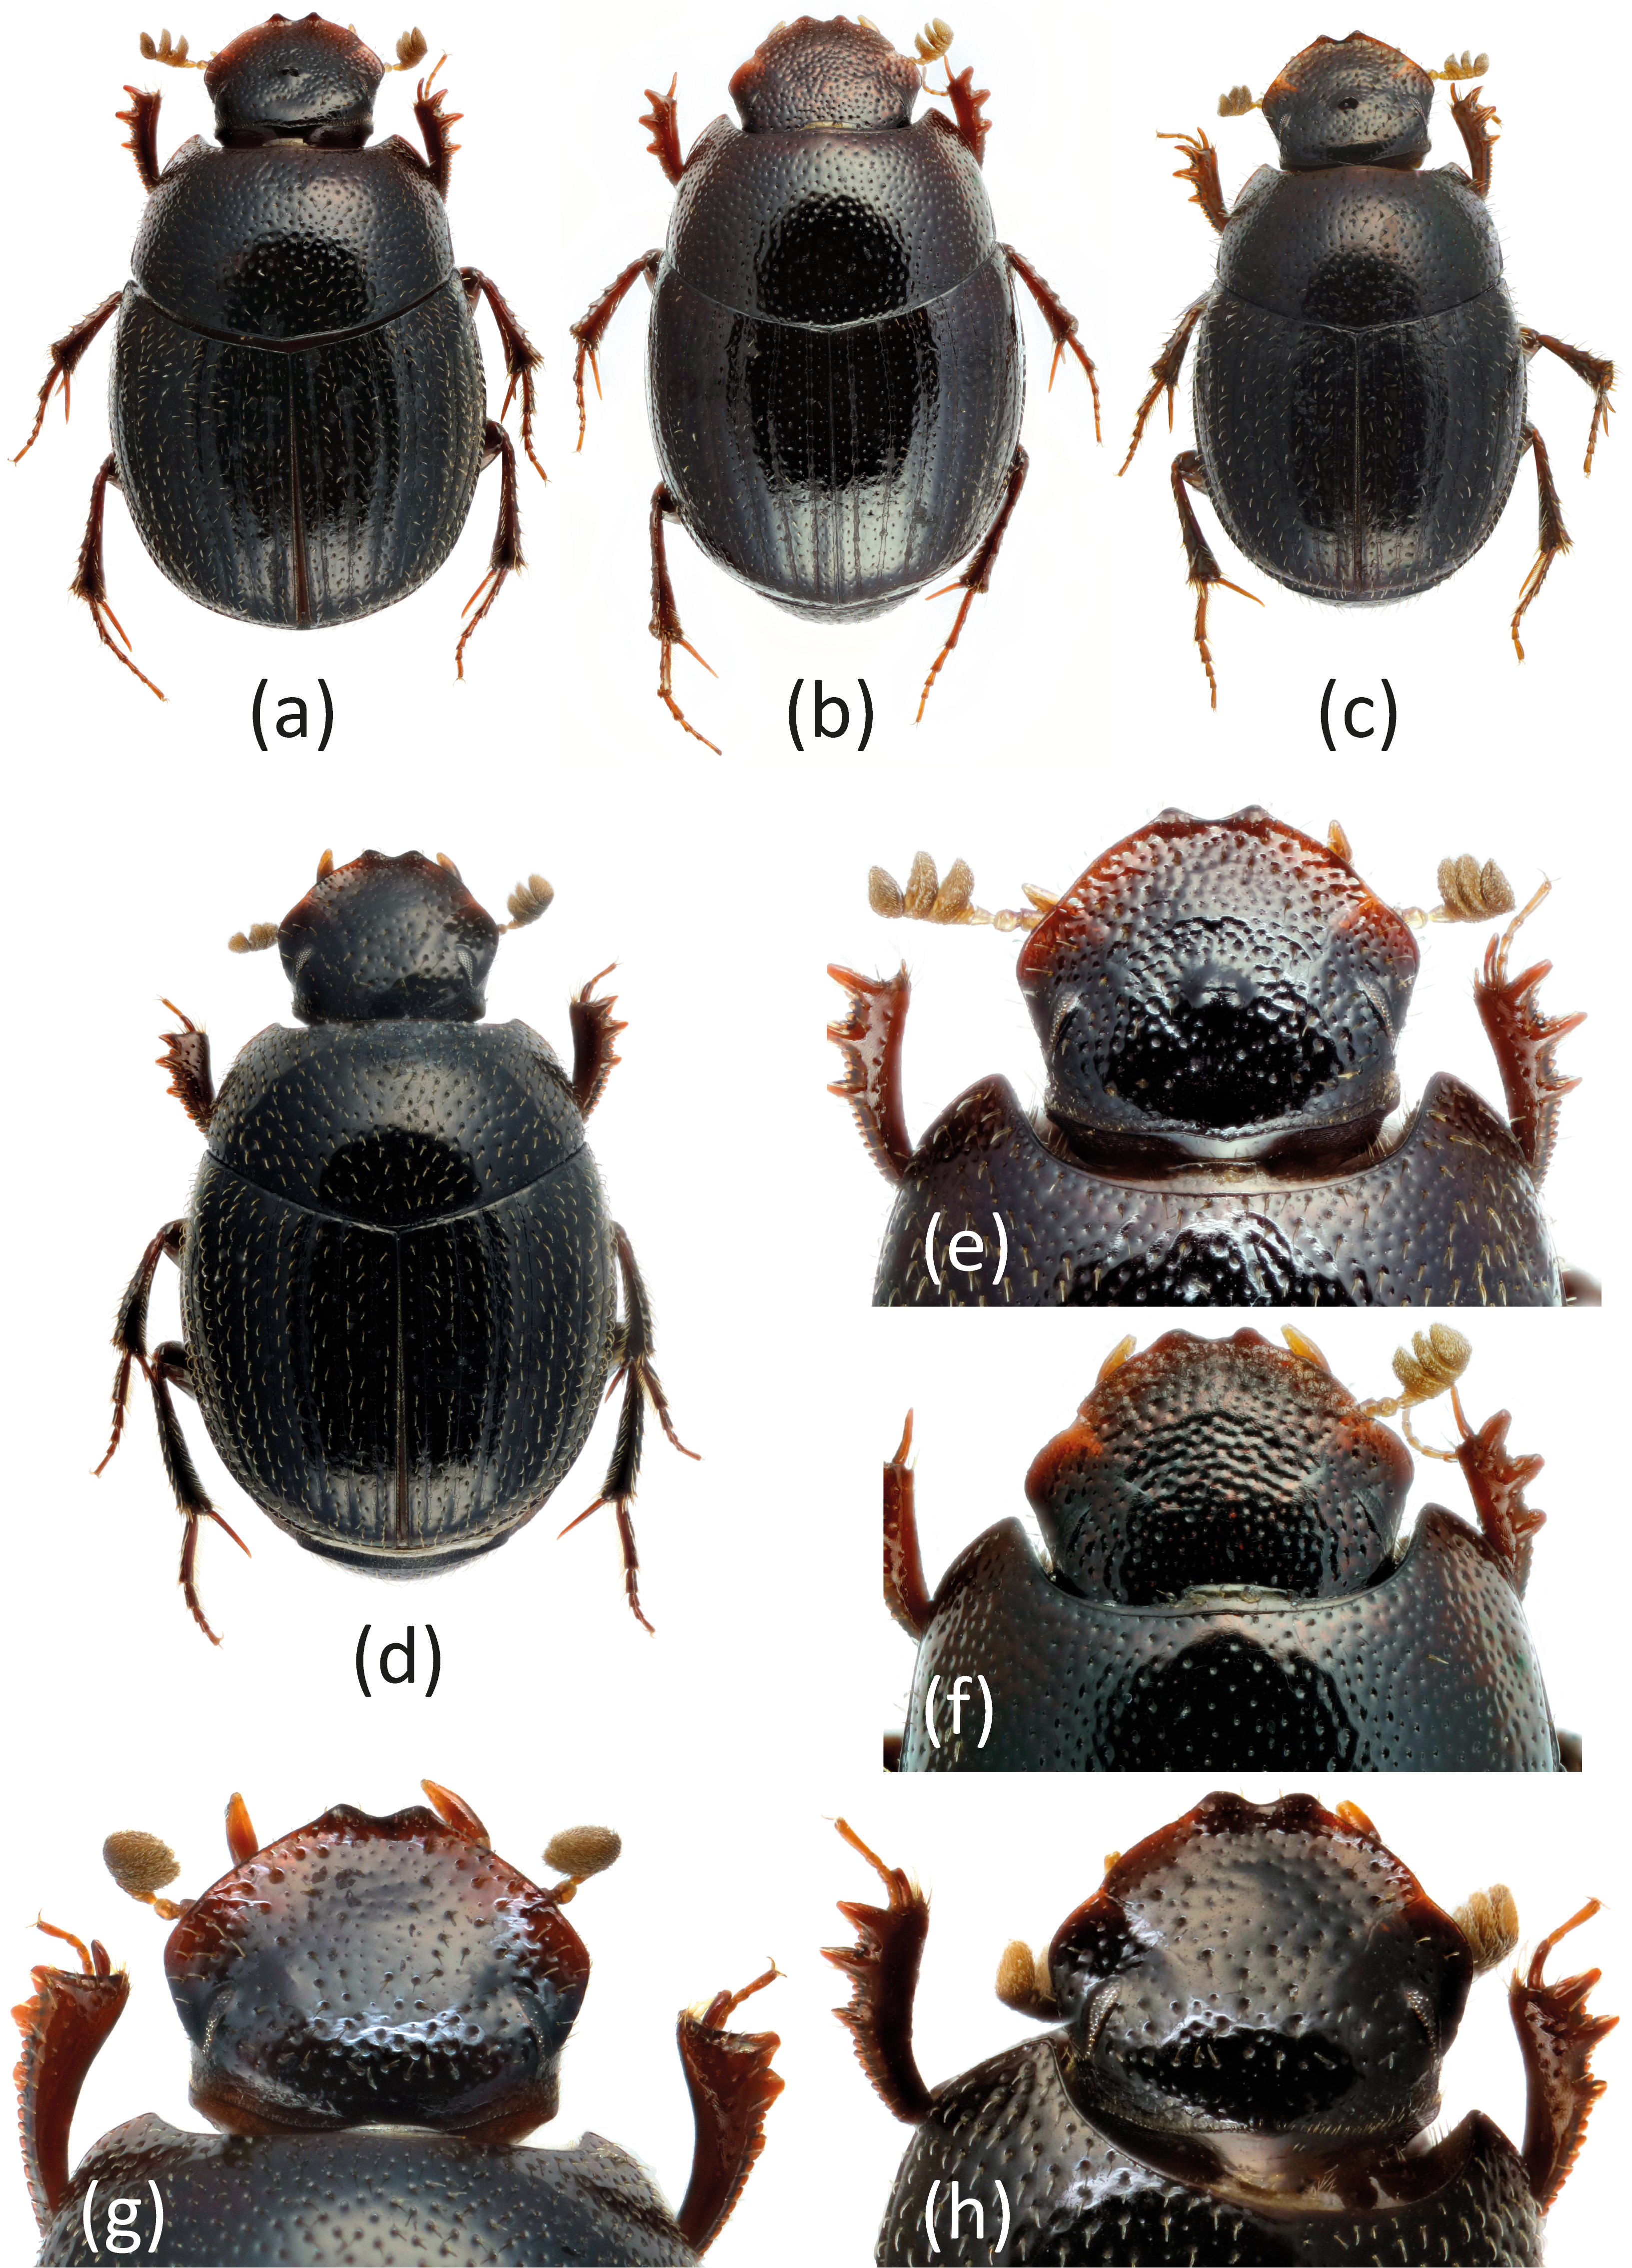
\includegraphics[width=\linewidth]{figure_1.jpg}
\caption{External morphology of \textit{Amietina} species. \textit{A. mazumbaiensis}: male (a) and female (b) habitus; male (e) and female (f) forebody. \textit{A. grebennikovi}: male habitus (c). \textit{A. larrochei}: male habitus (d) and forebody (h). \textit{A. eburnea}: male forebody (g).}
\label{fig:fig1}
\end{figure}

\begin{figure}[ht]
\centering
\includegraphics[width=\linewidth]{figure_2.jpg}
\caption{Genitalia of \textit{Amietina} species. \textit{A. mazumbaiensis}: aedeagus in lateral (a) and dorsal (b) views, blue arrow pointing at parameral posterolateral notch; endophallus (c); lamella copulatrix (LC) (l). \textit{A. grebennikovi}: aedeagus in lateral (d) and dorsal (e) views; endophallus (f); LC (m). \textit{A. larrochei}: aedeagus in lateral view (g); endophallus (h); LC (n). \textit{A. eburnea}: aedeagus in lateral view (i); endophallus (j). \textit{A. cambeforti}: aedeagus in lateral view (k).}
\label{fig:fig2}
\end{figure}

\begin{figure}[ht]
\centering
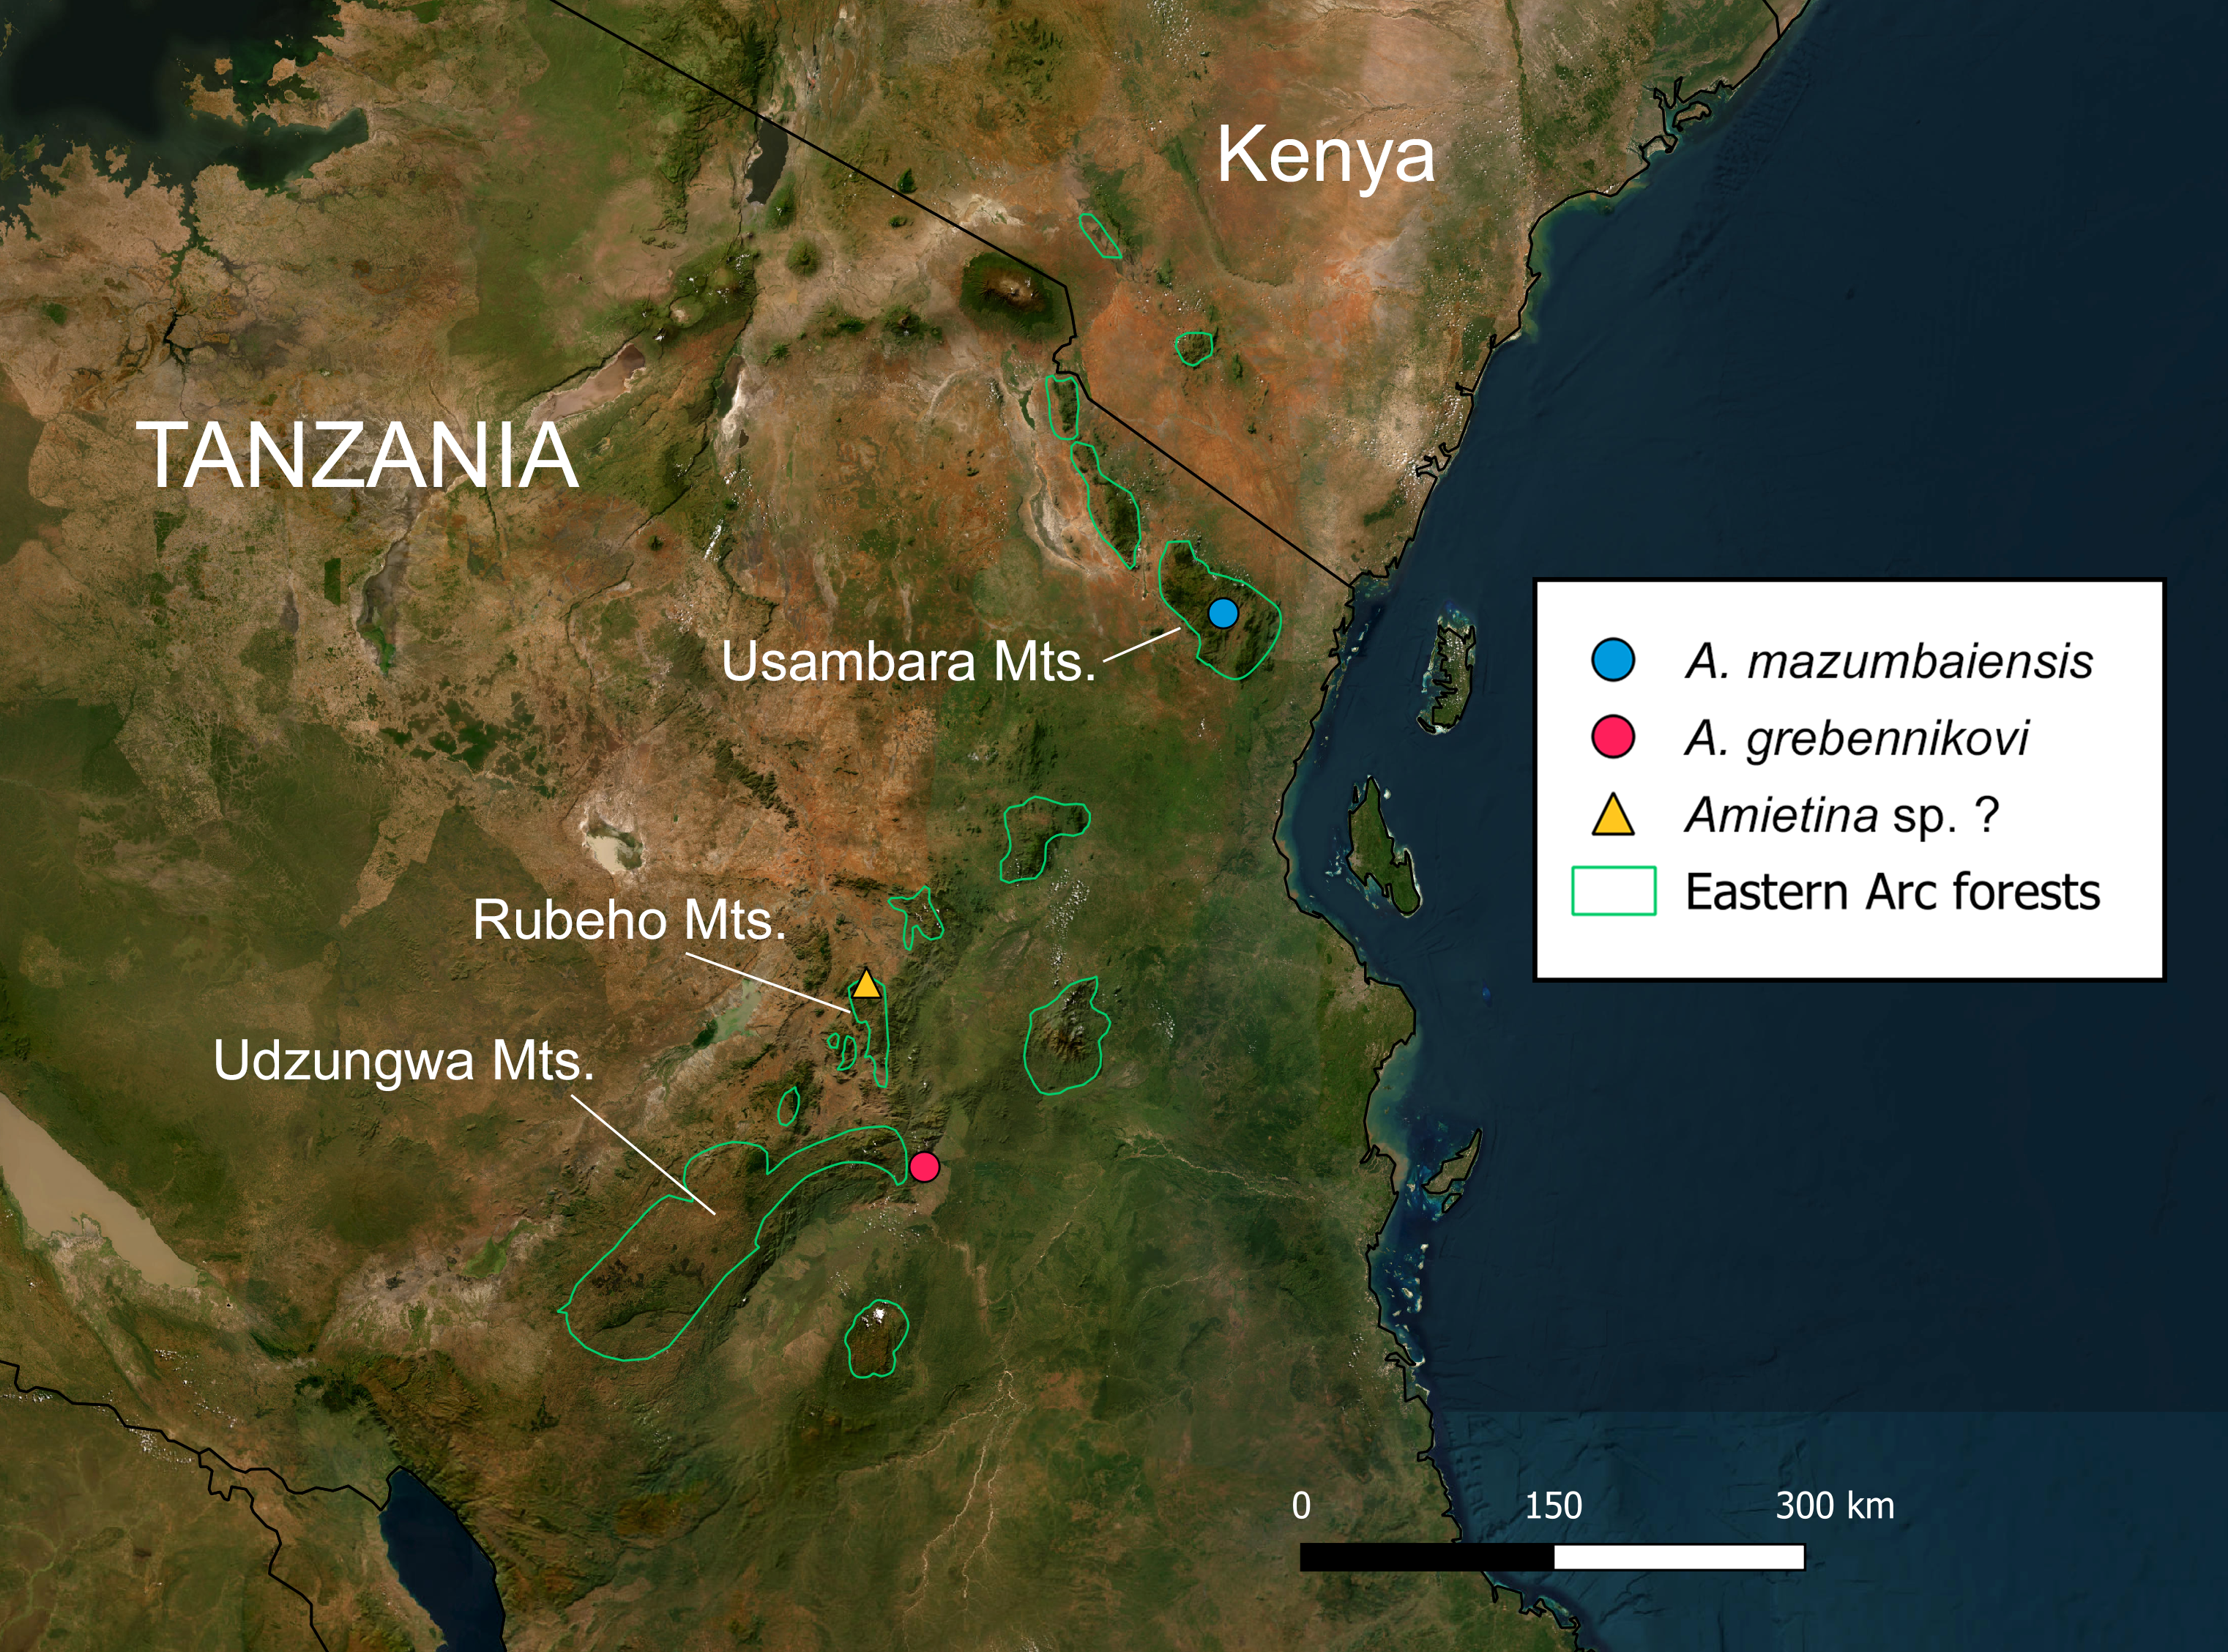
\includegraphics[width=\linewidth]{figure_3.png}
\caption{Distribution of \textit{Amietina} species in the Eastern Arc Mountains.}
\label{fig:fig3}
\end{figure}

\bibliography{sample}

\end{document}